\documentclass[conference]{IEEEtran}

\usepackage{cite}
\usepackage{booktabs}
\usepackage{fancyvrb}
\usepackage{graphicx}
\usepackage{url}

\begin{document}

\title{The Polyglot's Dilemma: Conformance Testing a Dozen Specs in as Many Languages}

\author{
  \IEEEauthorblockN{A. Jesse Jiryu Davis\IEEEauthorrefmark{1},
  Jeremy Mikola\IEEEauthorrefmark{2},
  and Jeff Yemin\IEEEauthorrefmark{1}}
  \IEEEauthorblockA{\IEEEauthorrefmark{1}MongoDB,
  New York, New York, USA\\
  \{jesse, jeff.yemin\}@mongodb.com}
  \IEEEauthorblockA{\IEEEauthorrefmark{2}Independent Researcher\\
  jmikola@gmail.com}
}

\maketitle

\begin{abstract}
MongoDB maintains client libraries in a dozen programming languages, used by tens of thousands of organizations and millions of developers. Most are implemented natively rather than as wrappers around a shared core. Ensuring consistent behavior across these libraries, comprising millions of lines of code, is hard but essential. Over eleven years, we developed a specification-based testing approach: tests are written once in YAML and executed by language-specific interpreters for each library. We describe the evolution from many ad-hoc formats to a Unified Test Format, which allowed us to delete over 12,000 lines of test code. We report lessons learned about declarative test design, test architecture, schema evolution, and the limits of unification.
\end{abstract}

\begin{IEEEkeywords}
conformance testing, domain-specific test language, polyglot development, MongoDB
\end{IEEEkeywords}

\section{Introduction}

Database client libraries are often implemented as thin wrappers around a shared core written in C. This architecture minimizes duplication, but shared-core libraries impose costs on users. Compiling and installing a C dependency is unfamiliar for many programmers, the library cannot participate in language-native async event loops, and its API rarely feels idiomatic.

At MongoDB, we chose a different path. We maintain approximately twelve client libraries (the number has changed over time), which we call ``drivers.'' We wrote the entire driver logic and API nine times in C, C\#, Go, Java, Node.js, Python, Ruby, and Rust. In addition, we wrote idiomatic layers in C++ and PHP that wrap the C Driver, and in Scala and Kotlin wrapping the Java Driver. This approach lets each driver integrate naturally with its ecosystem---it is easy to install, obeys native logging conventions, cooperates with async event loops, and presents an API that feels familiar to developers in that language. The cost is that we maintain the same client-server protocol, connection pooling, server discovery, and other behaviors in at least nine code bases.

Prose specifications help, but natural language is ambiguous. Differential testing~\cite{mckeeman_differential_1998} can detect how implementations diverge, but it cannot say which implementation is correct. It also cannot detect when all implementers make the same mistake---so-called common-mode failures---because the spec is unclear or because some errors are easy to make~\cite{brilliant_consistent_1987}.

Our solution is a \emph{domain-specific test language}, or DSTL: we write machine-executable tests in YAML that encode the spec author's intent. Each driver implements a test runner that interprets these YAML files, runs the specified operations against a MongoDB deployment, and asserts that the results match expectations. When specs change, we update the YAML tests in a central repository, and the changes propagate automatically to the individual drivers.

Starting in 2015, we developed and refined this approach. Our early efforts produced multiple test formats, each tailored to a particular specification: one DSTL for CRUD operations, another for transactions, another for connection pooling, and so on. By 2020, this proliferation had become a maintenance burden. We consolidated these formats into a Unified Test Format (UTF), validated by a JSON Schema. By migrating to UTF we deleted over 12,000 lines of redundant test-runner code, while gaining schema validation and a more expressive test language.

UTF introduced several mechanisms that we will explain in detail below. An \emph{entity map} is a registry of objects---clients, databases, collections (i.e.\ database tables), cursors---created during a test, allowing operations to reference them by name later in the test. \emph{Command monitoring} captures every message the driver sends to the server and every reply it receives, enabling tests to check wire-level behavior. \emph{Fail points} are server-side hooks that simulate errors, dropped connections, and slow responses, providing controlled conditions for testing error handling.

This paper reports on eleven years of industrial experience applying this methodology across a dozen driver implementations, comprising millions of lines of production code. Our drivers are used by tens of thousands of customers and millions of open source users. Even subtle inconsistencies in their behaviors are costly. While our techniques are not novel compared to recent research prototypes, we offer something complementary: empirical evidence that declarative, cross-language conformance testing scales to production systems over extended timeframes. We report what worked, what did not, and where we reached the limits of unification.

\begin{figure}[t]
    \centering
    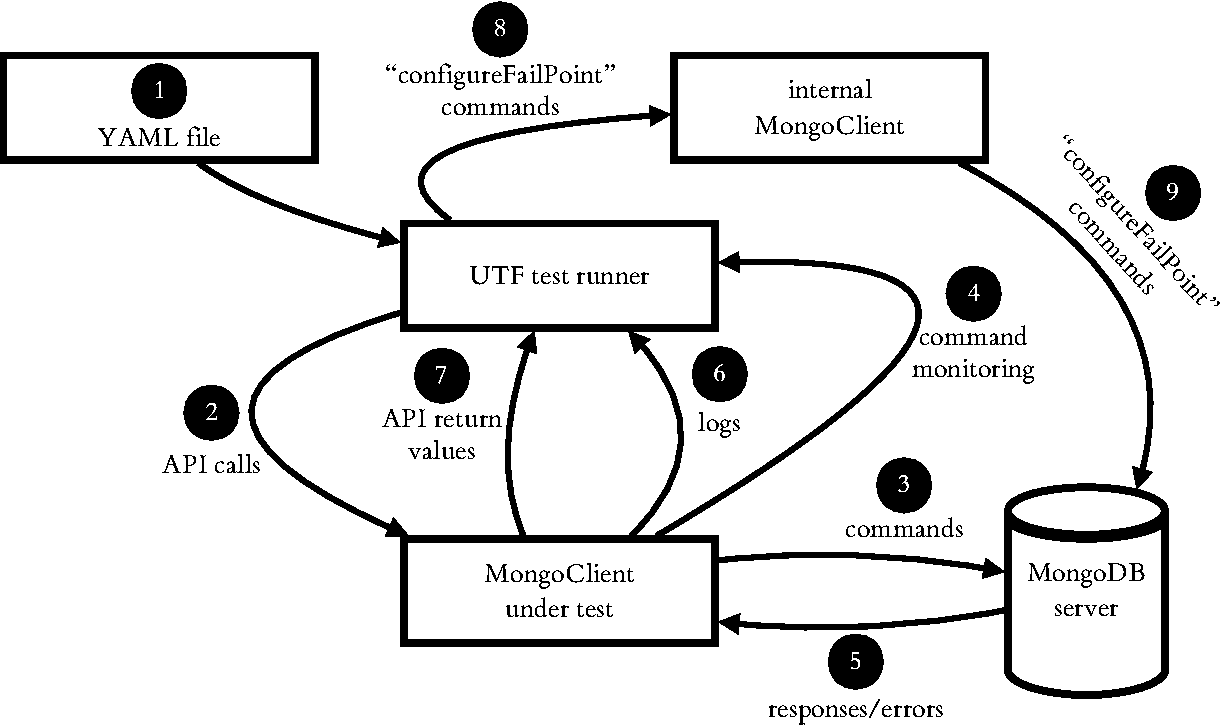
\includegraphics[width=\columnwidth]{FIG/test-architecture.key.cropped.pdf}
    \caption{MongoDB driver specification testing architecture.}
    \label{fig:architecture}
\end{figure}

\section{Test architecture and components}

The components for testing a MongoDB driver in any language with UTF are shown in Fig.~\ref{fig:architecture}. The UTF test runner reads a YAML file (1), and creates two client objects (MongoClients): a MongoClient under test, and an internal MongoClient for out-of-band communications with the MongoDB server. The test runner executes the YAML file's list of operations. For each operation it calls a method on the MongoClient under test (2), which sends commands to the server (3), and also reports them back to the test runner (4) via the command monitoring API. The server responds to the client (5), which may log to a file-like stream created by the test runner (6), and finally the original API call returns a value or error (7). The YAML file's operations may include fail points that the test runner should enable or disable to control the server's behavior; these are interleaved with other test operations. The test runner sends \texttt{configureFailPoint} commands to the server via its internal MongoClient to avoid interference.

The command monitoring API was designed for application performance monitoring (APM), but we quickly learned its value for testing drivers' network messages. Fail points are also vital: the server can be configured to return a certain error the next time a certain command is called, or to do so a certain number of times, or to block the command for a certain period, or close the connection. (A proxy server might serve the same purpose, at the cost of maintaining another component.)

Fig.~\ref{fig:utf-example} shows a complete test file in UTF. The test creates a client, database, and collection as named \textit{entities}, which are referenced by later operations using YAML anchors. The test populates a collection with initial data, then attempts a \texttt{replaceOne} operation. The driver should reject it: \texttt{\$set} is allowed in \texttt{updateOne} but not \texttt{replaceOne}. The \texttt{expectEvents} block asserts that no commands were sent to the server, because the driver detected the error client-side. Finally, \texttt{outcome} confirms the collection is unchanged.

\begin{figure*}[t]
\begin{minipage}[t]{0.48\textwidth}
\begin{Verbatim}[fontsize=\small, frame=single]
schemaVersion: "1.0"
createEntities:
  - client:
      # "&client0" defines an anchor.
      id: &client0 "client0"
      observeEvents:
        - "commandStartedEvent"
  - database:
      id: &database0 "database0"
      # "*client0" refers to the anchor.
      client: *client0
      databaseName: &db0Name "db"
  - collection: # a table in "db"
      id: &collection0 "coll"
      database: *database0
      collectionName:
        &coll0Name "test-coll"
initialData:
  - collectionName: *coll0Name
    databaseName: *db0Name
    documents:
      - { _id: 1, x: 11 }
\end{Verbatim}
\end{minipage}
\hfill
\begin{minipage}[t]{0.48\textwidth}
\begin{Verbatim}[fontsize=\small, frame=single]
tests:
  - description: "ReplaceOne prohibits
                  atomic modifiers"
    operations:
      - name: "replaceOne"
        object: *collection0
        arguments:
          filter: {_id: 1}
          replacement: {$set: {x: 2}}
        expectError:
          isClientError: true
    expectEvents:
      - client: *client0
        events: []
    outcome:
      - collectionName: *coll0Name
        databaseName: *db0Name
        documents:
          - { _id: 1, x: 11 }



\end{Verbatim}
\end{minipage}
\caption{A UTF test file. Left: entity definitions and initial data. Right: test operations and assertions.}
\label{fig:utf-example}
\end{figure*}

\section{Evolution of the Unified Test Format}

\subsection{Choosing YAML for writing specification tests}

We first introduced cross-driver test files with our Server Discovery and Monitoring (SDAM) specification in 2014. These tests checked drivers' behavior when connecting to a MongoDB cluster and responding to topology changes (e.g.\ a change in the number of servers in a consensus group~\cite{schultz_design_2022}). A test runner fed simulated server messages to a driver's internal state machine and asserted on its state transitions.

We considered the Cucumber testing framework, with its English-like Gherkin syntax. But Gherkin is intended to express business logic to non-programmers. Describing binary formats and TCP/IP connections was inconvenient and silly-looking; our engineers rebelled at the proposal. We settled on YAML for its programmer-friendly syntax, support for comments, and the availability of parsing libraries in most target languages. YAML allows basic factoring with \textit{anchors} and \textit{aliases}. Test files could be converted to JSON for languages that lack a YAML parser. The payload of most MongoDB wire protocol messages is BSON, a JSON-like binary format. Since YAML is a superset of JSON, payloads could be naturally embedded in YAML files. In 2017, we developed a MongoDB Extended JSON format that is valid JSON and converts losslessly to and from BSON.

These first YAML tests and all the drivers' test runners were specific to the SDAM spec. Guidelines for authoring tests in the DSTL and implementing a test runner were communicated in an appendix to the specification. The workflow for developing an SDAM test was: amend or create a YAML file in the specifications Git repository; convert all YAML test files to JSON; sync YAML and/or JSON test files to each driver's Git repository; and run the tests as part of continuous integration (CI).

Following SDAM, other specifications began to adopt YAML tests. By 2015 we had various DSTLs and test runners for driver functionality ranging from connection string parsing, to BSON serialization, to server selection. The CRUD spec, which defined APIs for read and write operations, introduced a DSTL for functional testing that would eventually be the foundation of UTF.

\subsection{CRUD v1: our first DSTL for testing driver APIs}

The initial DSTL for the CRUD specification (CRUD v1) allowed a driver to execute a single operation and assert either a \texttt{result} which must match a pattern in the YAML test, or an error. The test runner could also assert the final state of the database collection under test, which might have been pre-loaded with data fixtures before the test and/or modified by a write operation.

Fig.~\ref{fig:crud-v1-example} is a YAML test for a driver's \texttt{insertOne} method, which returns the primary key of the inserted document. Early tests used explicit values for primary keys (the \texttt{\_id} key) instead of driver-generated unique ids. At the time, the DSTL offered no syntax for matching dynamic values; fixed values allowed for predictable assertions on the operation result and collection under test.

\begin{figure*}[t]
\begin{minipage}[t]{0.48\textwidth}
\begin{Verbatim}[fontsize=\small, frame=single]
data: [{ _id: 1, x: 11 }]
tests:
  - description: "InsertOne with a
                  non-existing document"
    operation:
      name: "insertOne"
      arguments:
        document: { _id: 2, x: 22 }
\end{Verbatim}
\end{minipage}
\begin{minipage}[t]{0.48\textwidth}
\begin{Verbatim}[fontsize=\small, frame=single]
    outcome:
      result:
        insertedId: 2
      # Expected final contents of table
      collection:
        - { _id: 1, x: 11 }
        - { _id: 2, x: 22 }

\end{Verbatim}
\end{minipage}
\caption{A CRUD v1 test file.}
\label{fig:crud-v1-example}
\end{figure*}

Compare this to the UTF example in Fig.~\ref{fig:utf-example}: the single implicit collection is replaced there by explicit entities, and the \texttt{outcome.collection} field becomes a more general \texttt{outcome} array.

CRUD v1 provided little guidance on how test runners should match documents in the collection under test to their expected values, or match an API result to its expected value. Later test formats would give this subject more attention as we stumbled over edge cases. Eventually, UTF went so far as to define rules for numeric comparisons between 32-bit and 64-bit BSON integers.

\subsection{Command monitoring}

In 2015 we specified a \textit{command monitoring} API for drivers, allowing applications to observe every message between the driver and the server. The test format for command monitoring extended the CRUD v1 DSTL with an \texttt{expectations} field for each test, which contained an ordered list of event objects to be observed and matched (renamed \texttt{expectEvents} in UTF). Most operations produce one CommandStartedEvent followed by either a CommandSucceededEvent or CommandFailedEvent. For example, a successful \texttt{insertOne} operation would first expect a CommandStartedEvent containing an outgoing command encoded in BSON, followed by a CommandSucceededEvent containing a BSON server response.
Slight variations in client-side BSON encoding and server responses (across versions and topologies) would become an emerging concern for test authors.

\subsection{Retryable reads and writes: we start using server fail points}

MongoDB introduced a protocol to idempotently retry failed read and write operations in 2017. The MongoDB server already had an internal \texttt{configureFailPoint} command for scheduling errors to aid with end-to-end testing; we began to use this feature systematically in driver testing as well. Our YAML format for testing retryable reads and writes could instruct the test runner to set a fail point before running an operation.

\subsection{Transactions: error assertions and dynamic matching}

In 2018, MongoDB introduced support for transactions, and our YAML tests for transactions made heavy use of fail points. To test sharded transactions, we added the ability to configure fail points on specific servers in the sharded cluster. We also needed more complex assertions between operations, e.g.\ to check the current transaction state. This prompted the creation of ``special test operations,'' which were specified within the list of operations but invoked an arbitrary function on the test runner instead of a method on the database or collection object under test.

Below, a special test operation asserts the state of a transaction associated with one of two session objects managed by the transactions test runner (``session0'' or ``session1''):

\begin{Verbatim}[fontsize=\small, frame=single]
- name: assertSessionTransactionState
  object: testRunner
  arguments:
    session: session0
    state: in_progress # assertion
\end{Verbatim}

Earlier DSTLs had only basic assertions for operation results and errors. A \texttt{result} assertion could expect a scalar value, BSON document, or sequence of documents, but an \texttt{error} assertion merely checked that the operation had failed. Error reporting was a crucial design element of the transactions specification. The server's error messages now included \textit{labels} providing context and indicating whether it was safe to retry the transaction. We added richer error assertions to the DSTL to examine error labels, messages, and numeric codes.

Transaction tests also needed some way to match dynamic values, such as logical session IDs, in observed command events. UTF would eventually introduce special matching operators for test runners (e.g.\ \texttt{\$\$type}, \texttt{\$\$sessionLsid}), but earlier approaches were more primitive. For instance, the transaction test runner interpreted an expected value of 42 as a wildcard when matching a timestamp in an observed server response. Test authors would recognize 42 as special if they had read the DSTL documentation, or the Hitchhiker's Guide to the Galaxy~\cite{adams1979hitchhiker}.

\subsection{CRUD v2: one last milestone}

As DSTLs for other specifications were evolving over four years, any new tests for the CRUD specification were still written using the original v1 format, which was largely unchanged since 2015. In 2019, there was an effort to modernize the CRUD DSTL with a v2 edition. We introduced support for multiple operations, and for matching outgoing requests via command monitoring. This was an opportunity to codify matching logic (for checking that a result or collection matched its expected value), which had been undocumented.

\section{Unified Test Format}

UTF debuted in 2020 with a reenvisioned DSTL, backed by a JSON schema and a thoroughly specified test runner. It superseded all previous formats in the lineage dating back to CRUD v1 (Fig.~\ref{fig:lineage}). Fig.~\ref{fig:utf-example} is an example of the mature format.

There are 28 revisions to the UTF schema to date. Old files validate with the latest schema, and the newest test runners can interpret the oldest files. Each UTF file includes a top-level \texttt{schemaVersion} field, which specifies the JSON schema version to which the file conforms. This serves two purposes. First, a test runner can determine at a glance if it is capable of interpreting the file. Second, the CI tests for the specifications repository can validate each test file against its schema. Since development of drivers' test runners typically trails that of UTF, test authors try to use older \texttt{schemaVersions} to maximize compatibility.

Previous test formats used several top-level fields to restrict test execution (e.g.\ \texttt{minServerVersion}, \texttt{topologies}), which were evaluated as a single logical conjunction (i.e.\ ``and''). UTF replaces those fields with a single \texttt{runOnRequirements} array field containing one or more sets of conjunctive criteria. If at least one set of criteria is satisfied, the test runs.

\begin{Verbatim}[fontsize=\small, frame=single]
# Non-sharded transactions: 4.0; full: 4.2
runOnRequirements:
  - { minServerVersion: '4.0',
      topologies: [ replicaset ] }
  - { minServerVersion: '4.2',
      topologies: [ sharded ] }
\end{Verbatim}

In previous test runners, a fixed set of objects were created during setup and implicitly referenced by test operations. For example, a CRUD test operation would assume the single collection object under test. The UTF runner institutes a general-purpose object registry: the entity map. Entities can be explicitly defined in the \texttt{createEntities} section of a test file and later referenced by name in test operations (use of YAML anchors and aliases is encouraged, as seen in Fig.~\ref{fig:utf-example}).

Using the entity map, a single test can now create multiple collections with different options and interact with them individually. Additionally, the \texttt{saveResultAsEntity} syntax saves operation results to the entity map so they can be referenced later in the test.

Like CRUD v2, UTF specifies rules for matching logic in great detail. Notable rules include:

\begin{itemize}
\item Flexible comparisons for numeric types (generally following server behavior)
\item Selectively ignoring optional fields in BSON documents
\item Ignoring key order when comparing documents (BSON is ordered, YAML/JSON are not)
\item Special operators for complex assertions (e.g.\ asserting whether a field exists, asserting its type, matching against a dynamic value stored in the entity map).
\end{itemize}

\begin{figure}[t]
    \centering
    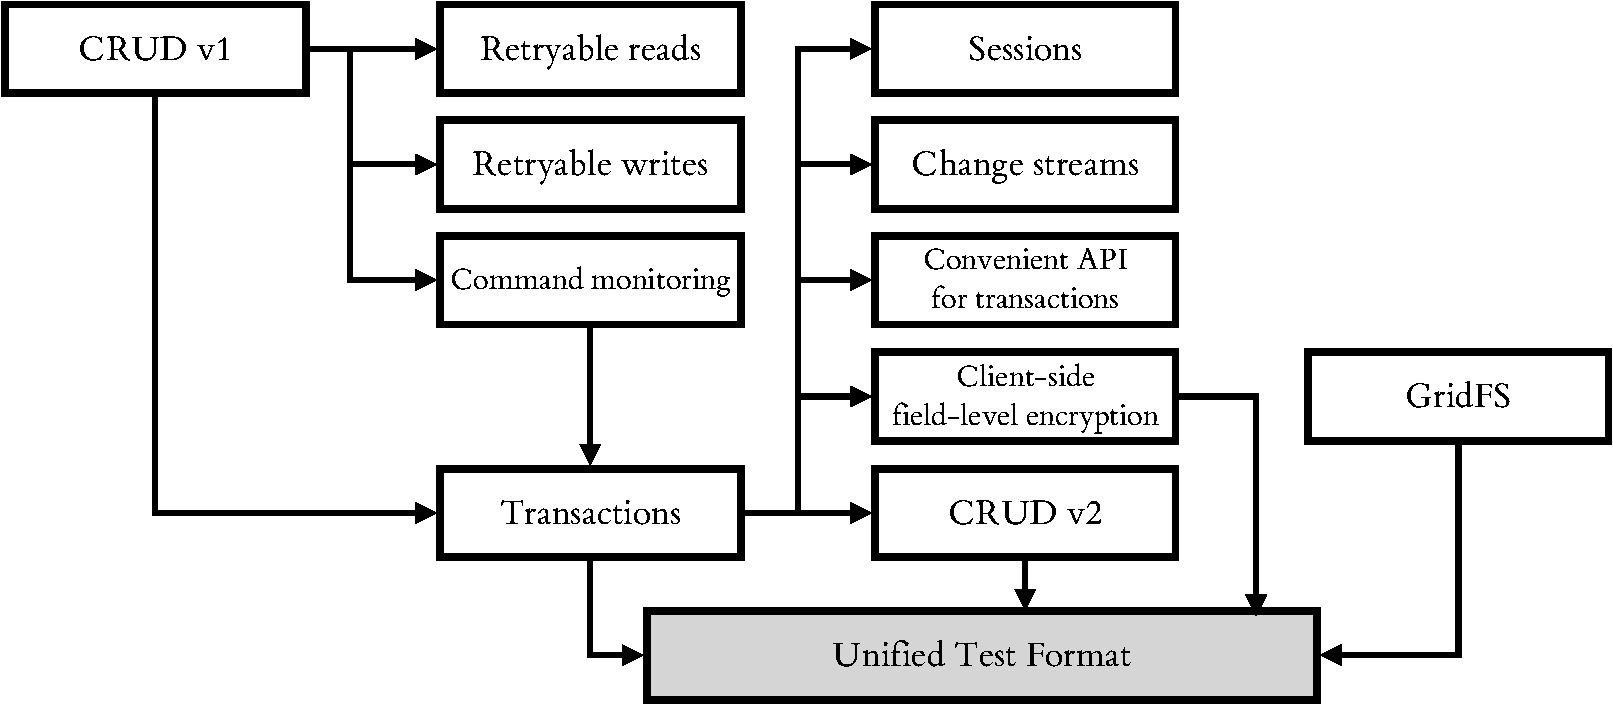
\includegraphics[width=\columnwidth]{FIG/format-lineage-2.key.cropped.pdf}
    \caption{Lineage of YAML test formats (including some not discussed in this paper).}
    \label{fig:lineage}
\end{figure}

When we first designed UTF we manually ported a sample of existing tests, to prove UTF covered all our requirements. Once UTF was formalized, we wrote one-off scripts for each legacy test format to mechanically convert it to UTF.

\subsection{Notable schema changes to UTF since inception}

UTF has evolved since 2020. There have been 28 revisions to its JSON schema and, although some syntax has been deprecated, no syntax has been removed. Tests written against the earliest schema versions can still be executed by the current version of the test runner.

In addition to command monitoring, MongoDB drivers support event-based monitoring of other internal mechanisms such as server discovery (SDAM) and connection pooling. Although the first version of UTF supported only command monitoring assertions in its \texttt{expectEvents} syntax, a forward-thinking design required minimal changes when incorporating new connection pooling and SDAM event types in later versions. Specification authors attempt to work within the existing schema, or make the smallest enhancement needed. When we added SDAM testing to UTF, we needed a way to run operations concurrently. We defined a new ``thread'' entity type and associated operations with threads (e.g.\ ``waitOnThread'', ``runOnThread''), which allowed new SDAM tests to reuse the old \texttt{operations} syntax.

Testing for standardized logging did warrant a new top-level \texttt{expectLogMessages} field; however, it was closely modeled after \texttt{expectedEvents} and thus required minimal test runner changes. We used a similar approach when introducing the \texttt{expectTracingMessages} syntax to test drivers' OpenTelemetry integration.

\begin{figure}[t]
    \centering
    \begin{minipage}{0.48\columnwidth}
        \centering
        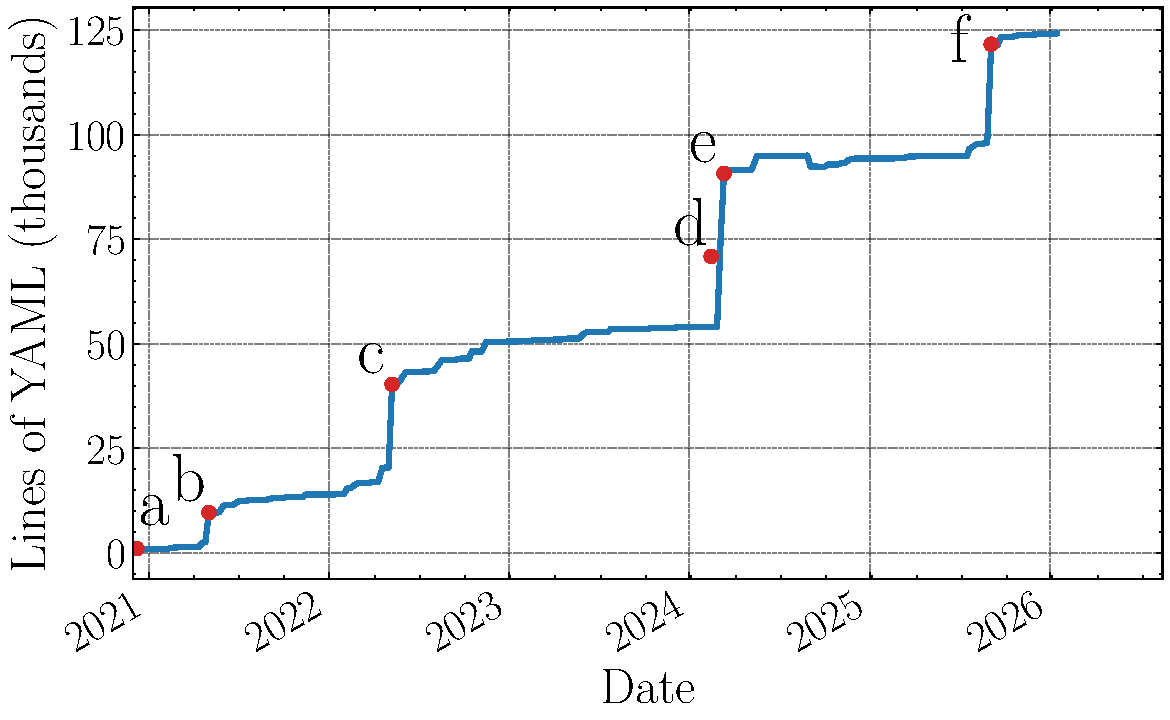
\includegraphics[width=\linewidth]{FIG/count_utf_lines.pdf}
        \caption{Unified Test Format corpus growth.}
        \label{fig:count_utf_lines}
    \end{minipage}
    \hfill
    \begin{minipage}{0.48\columnwidth}
        \centering
        
\includegraphics[width=\linewidth]{FIG/utf_driver_code_changes.pdf}
        \caption{Lines deleted from drivers' test code during UTF migration.}
        \label{fig:utf_driver_code_changes}
    \end{minipage}
\end{figure}

\subsection{Process for developing new specifications and tests}

The technical requirements for MongoDB drivers are defined across dozens of specifications, which are maintained in a Git repository alongside UTF. When creating or modifying a specification with accompanying UTF tests, the author must determine whether new syntax or test runner behavior is required. If so, changes to UTF will be made simultaneously and implemented in drivers alongside any spec change(s). Typically, new spec changes will be prototyped in at least two to three drivers before being published for wider adoption.

Historically, MongoDB engineers manually synced YAML tests from the specs repository into drivers' repositories. Beginning in 2024, several drivers transitioned to including the specs repository as a Git submodule. We configured GitHub's Dependabot to automatically create pull requests to update the submodule weekly. If CI reports that the driver's test suite passes with the test changes, the pull request is automatically merged. Since test runners skip files with an unsupported \texttt{schemaVersion}, there is generally no issue with updating test files before a driver can implement the latest specs and test format changes.

\section{Results}

Since 2020 our corpus of UTF tests has grown from a prototype with 7 files and 1046 lines of non-comment non-whitespace YAML, to 606 files with 124,168 lines. Fig.~\ref{fig:count_utf_lines} shows the major events in UTF's growth: we created UTF (a), ported the CRUD v2 tests (b), added Client-Side Operations Timeout tests (c), ported transactions tests (d), ported remaining CRUD v1 and retryable writes/reads tests (e), and ported CSFLE (f). Most drivers have replaced most of their runners for the various test formats in favor of one UTF runner, and they deleted test code on net. The Rust driver had the most dramatic savings of 4066 LOC (Fig.~\ref{fig:utf_driver_code_changes}).

\subsection{Testing the UTF test runner and its tests}

The UTF test runner has its own set of tests, which are divided into three categories: ``invalid'' test files are expected to fail JSON schema validation, ``valid-fail'' test files should pass schema validation but fail at runtime (e.g.\ an assertion failure), and ``valid-pass'' tests should pass without error. Collectively, these tests can assert correctness of the JSON schema. The set of ``valid-fail'' and ``valid-pass'' tests can additionally be used to verify correctness of a driver's test runner.

Automated checks on GitHub pull requests catch a number of mistakes that were common prior to UTF. YAML files are validated against their declared JSON schema version and a secondary check ensures that YAML and JSON files are in sync with one another (i.e.\ the pull request did not neglect to regenerate JSON files).

\subsection{Lessons Learned}

\textbf{We cannot unify everything:} UTF is not suitable for every spec. We still have specialized YAML formats and runners for testing BSON serialization, the SDAM state machine, connection string parsing, and other features. Some tests are simply described in English. If our YAML format were capable of describing any possible test, it would have become a Turing-complete programming language with interpreters in a dozen other languages, and its cost and risks would outweigh the benefits. We stopped folding formats into UTF when we reached the point of diminishing returns.

\textbf{Single schema version:} UTF's monotonically increasing schema version led to situations where a driver was blocked from implementing the tests for a new spec, because it had fallen several schema versions behind. If UTF files instead had a list of required test runner features, driver engineers would have had more flexibility about the order in which they implemented specs.

\textbf{Judicious enforcement:} Despite spec authors' efforts, our drivers still have some implementation-specific behavior. For example, a field on a result/response object might be optional or absent in some drivers. We added the \texttt{\$\$unsetOrMatches} operator to UTF so that test authors can permit drivers \textbf{not} to return a value in some cases, but require a \textbf{specific} return value if there is one.

\section{Related Work}

Our task---implementing the same network protocol and a consistent API in many programming languages---falls within the category of \textit{multilanguage development}, defined as any methodology in which some tasks require code changes in more than one language~\cite{mussbacher_polyglot_2024}. The subcategory of \textit{polyglot programming} describes the development of an individual program with components in multiple languages; testing such programs is a well-studied problem~\cite{houdaille_polyglot_2024,yang_multi-language_2024}. However, testing the conformance of \textit{multiple} programs, each in a different language, has to our knowledge been investigated much less.

\subsection{Domain-specific test languages}

Our YAML tests are an example of a \textit{domain-specific test language}, or DSTL~\cite{felicio_rapitest_2023,da_silva_test_2019,dragoi_domain_2023,ye_automated_2021,smithy_authors_http_nodate}. For example, many telecommunication protocols' test suites are written in the TTCN family of DSTLs~\cite{grabowski_design_2000}. A well-known DSTL is Gherkin, an English-like language for writing scenarios in a structured Given--When--Then form. A test runner called Cucumber executes the scenarios. We rejected Gherkin because it is designed for communication with non-technical stakeholders, whereas our tests are by and for engineers.

The Smithy project includes a DSTL that is more like our YAML tests~\cite{smithy_authors_http_nodate}. Smithy is an interface definition language for services. Engineers write test cases in Smithy's DSTL which specify exactly how the client and server implementations should serialize RPCs on the wire as HTTP messages. Similar to our YAML tests, Smithy's DSTL tests interact with both a client's ``upper'' and its ``lower'' surface; i.e.\ both the in-process function-call API it presents to an application, and the messages it sends on the wire. Interpreters for Smithy's DSTL are available in at least nine languages.

Netrix~\cite{dragoi_domain_2023} is a DSTL for consensus protocols such as Raft and Tendermint. Such protocols are asynchronous and nondeterministic; an astronomical number of event sequences are possible in any test run. With Netrix, engineers write \textit{filters} which constrain the possible order of events, while still permitting some nondeterminism. For example, in ordinary execution it is possible but unlikely that all ``Prepare'' messages from some node \textit{n} are lost. An engineer can write a Netrix filter that drops all such messages, guiding execution toward some interesting set of behaviors. Netrix implements a proxy server that enforces filters, and a random fuzzer that explores behaviors within the filtered set.

Ecma International maintains a repository called Test262, containing over 50,000 handwritten test cases to check JavaScript implementations' conformance to the ECMA-262 standard~\cite{ye_automated_2021}. Each ``case file'' is written in a DSTL that must be interpreted by a complex test runner. The case file instructs the runner how to combine templates or include-files into an executable JavaScript test, whether to expect an exception, and other information. The same as MongoDB, Ecma wrote a spec of the spec tests, describing the case file format and how test cases should be run. There are at least six independent implementations of the Test262 spec; they can check the conformance of JavaScript runtimes embedded in Node, a web browser, a C++ program, and so on.

\subsection{Test Case Generation}
\label{test-case-generation}

MongoDB driver specifications are written in English, and we wrote our YAML tests by hand. But there are many examples of specifications that use formal logic, or some formal specification language, or a finite state machine (FSM). In these cases one can generate test cases mechanically with well-known techniques~\cite{richardson_approaches_1989}, especially in the realm of network protocols~\cite{hoque_ensuring_2015,mcmillan_formal_2019,mcmillan_compositional_2019,bishop_engineering_2006,singha_messi_2024,raghavan_protocol_1995,dssouli_test_1999}. Now, LLMs can generate test cases from natural-language specs as well. COMFORT~\cite{ye_automated_2021} is an experimental system that uses an LLM to generate JavaScript test cases from ECMA-262. The LLM benefits from ECMA-262's rigidly structured English. COMFORT's test cases do not include expected outputs; instead, COMFORT applies differential testing with many JavaScript implementations. If one implementation's output differs from all the others, it is probably wrong, and COMFORT flags it for human investigation.

\subsection{Testing the upper and lower surface}

A major strength of our approach is that we test not only the return values of API calls, but also the contents of drivers' messages on the wire. A survey by Bochmann et al.~\cite{bochmann_protocol_1994} mentions this possibility in the context of FSM-based conformance testing. The ``ferry-clip'' test architecture is a realization of this idea~\cite{chanson_design_1989}. It tests an implementation of an OSI protocol layer by controlling the protocols above and below it in the OSI stack, attaching to the SUT's top and bottom like a ``clip.'' The test harness installs a proxy server which ``ferries'' messages produced by the SUT back to the test harness to be checked against assertions. Our tests' mechanics are quite different---we use direct procedure calls at the top surface, and command-monitoring callbacks at the bottom---but the architecture is somewhat analogous.

\section{Future Work}

MongoDB driver engineers will continue adding features and making improvements to the drivers, in response to server changes or new client-side requirements. Therefore we will write more specs and more UTF tests, and (as rarely as possible) new versions of the UTF schema.

For the most part, UTF is \textit{example-based testing}: a human manually constructs inputs and expected results, one at a time. A few of our specs include scripts that generate UTF tests from data files and templates. In the future, we could explore our drivers' behavior far more thoroughly with \textit{property-based testing}, if we found a reasonable YAML syntax for generating inputs and checking the correctness properties of results. Property-based testing is especially powerful when combined with \textit{coverage-guided fuzzing}; this is a promising direction for further research.

We could also generate test inputs with any of the techniques in Section~\ref{test-case-generation}. E.g.\ we could model MongoDB's client-server system as an FSM, and check that the FSM's transitions match the drivers'. We could also use an LLM to generate more test files from the prose spec and existing tests. The LLM could autonomously check its work in an agentic loop: if every driver fails an LLM-made test, the test is probably wrong, but if only some fail, the test may have uncovered a bug. At the cutting edge, an LLM could generate a driver in a new programming language from the prose specs and UTF tests. Like humans, coding agents perform best when they have precise instructions and unambiguous correctness checks; we already have both.

\section{Conclusion}

We described a specification-based testing method developed over eleven years to ensure consistent behavior among libraries in a dozen languages, serving millions of users. We found that declarative, machine-interpretable test specs are effective at enforcing consistency. Our Unified Test Format minimizes the cost of maintaining tests: each driver implements a single UTF test runner; tests are written once and run everywhere. Our approach is not as advanced as some prior research, but its continuous use and evolution at scale offers an extended case study. We hope the lessons we learned prove useful to other teams enforcing consistent behavior across many implementations.

\bibliographystyle{IEEEtran}
\bibliography{references,other_references}

\end{document}
